\documentclass{beamer}

\usepackage[utf8]{inputenc}
\usepackage[T1]{fontenc}
\usepackage{lmodern}
\usepackage{graphicx}
\usepackage{amsmath}
\usepackage[french]{babel}
\usepackage{array}

%\usetheme{Hannover}
\usetheme{Madrid}

\title[Analyse de iSudoku]{Analyse de iSudoku}
\subtitle[\ldots]{Projet de l'UE Ingénierie du Logiciel}
\author{
  Maude \bsc{Bel}
  \and
  Antoine \bsc{Houssais}
  \and
  Théo \bsc{Lebourg}
  \and
  Jérôme \bsc{Rahault}
  \and
  Fabricio \bsc{Santolin Da Silva}
  \and
  Simon \bsc{Tchernia}
}
\institute{Université Pierre et Marie Curie}
\date{\today}

\AtBeginSection[] {
  \begin{frame}
    \frametitle{Sommaire}
    \tableofcontents[currentsection, hideothersubsections, pausesubsections]
  \end{frame}
}

\begin{document}

\maketitle

\section{Présentation du groupe et de l’organisation}
\subsection{Gestion partagée des modèles et du code}
\begin{frame}
  \frametitle{Gestion partagée des modèles et du code}
  \begin{description}
    \item [Notre hébergeur de projet] \url{htps://github.com/neir/iSudoku}
      \pause
    \item [Notre logiciel de gestion de versions] Git
\end{description}
\end{frame}
\section{Phase d’analyse du iSudoku}
\subsection{Diagramme de cas d’utilisation}
\begin{frame}
\frametitle{Diagramme de cas d'utilisation}
\begin{figure}[h]
  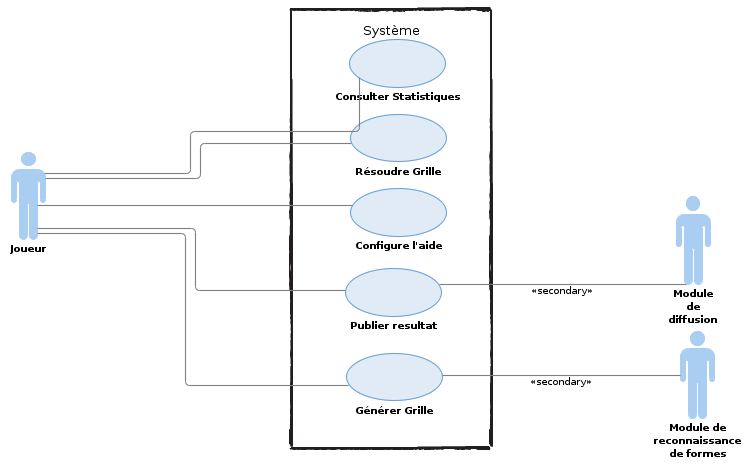
\includegraphics[scale=0.4]{diagrammeCasDUtilisation.png}
\end{figure}
\end{frame}
\subsection{Fiche détaillée de cas d’utilisations}
\begin{frame}
  \frametitle{Fiche détaillée du cas d'utilisation « Résoudre Grille »}
\begin{description}
  \item [But]
    L'utilisateur veut résoudre une nouvelle grille de sudoku
    \pause
  \item [Séquencement]
    Le cas d'utilisation commence lorsque la grille apparaît sur l'écran du
    smartphone / tablette
  \pause
  \item [Enchaînement nominal]
    \begin{enumerate}
      \setbeamertemplate{enumerate item}[circle]
    \item
      L'utilisateur sélectionne une case vide de la grille à remplir.
      \pause
    \item
      Le système affiche une aide selon le niveau de difficulté :
      \begin{itemize}
        \setbeamertemplate{itemize item}[circle]
        \item
          facile : le système affiche pour chaque case les valeurs possibles au vu du
          reste de la grille
        \item
          difficile : le système n'affiche rien
        \end{itemize}
      \pause
    \item
      L'utilisateur entre un numéro de 1 à 9 dans cette case.
      \pause
    \item
      L'utilisateur répète l'action 1) jusqu'à compléter intégralement la grille.
      \pause
    \item
      L'utilisateur valide la grille.
    \end{enumerate}
  \end{description}
\end{frame}
\end{document}
